% +------------------------------------------------------------------------+
% | CGAL User Manual: 
% +------------------------------------------------------------------------+
% |
% | 10.07.2008   Peter Hachenberger
% | 
\RCSdef{\MinkowskiSum3Rev}{$Id$}
\RCSdefDate{\MinkowskiSum3Date}{$Date$}
% +-----------------------------------------------------------------------+

\ccParDims

\ccUserChapter{3D Minkowski Sum of Polyhedra \label{chapterMinkowskiSum3}}
\ccChapterRelease{\MinkowskiSum3Rev. \ \MinkowskiSum3Date}
\ccChapterAuthor{Peter Hachenberger}


\begin{ccPkgDescription}{3D Convex Hulls\label{Pkg:ConvexHull3}}
\ccPkgHowToCiteCgal{cgal:hs-ch3-07}
\ccPkgSummary{This package provides functions 
for computing convex hulls in three dimensions as well as functions
for checking if sets of points are strongly convex are not. One can
compute the convex hull of a set of points in three dimensions in one
of three ways: using a static algorithm, using an incremental
construction algorithm, or using a triangulation to get a fully
dynamic computation.}

\ccPkgDependsOn{All algorithms produce as output a \ccRef[3D Polyhedron]{Pkg:Polyhedron}. 
                The dynamic algorithms depend on \ccRef[3D Triangulations]{Pkg:Triangulation3}}
\ccPkgIntroducedInCGAL{1.1}
\ccPkgLicense{\ccLicenseQPL}
\ccPkgIllustration{Convex_hull_3/bunny.png}{Convex_hull_3/bunny.png}
\end{ccPkgDescription}


% +------------------------------------------------------------------------+
\section{Introduction}

\begin{figure}[h]
  \begin{ccTexOnly}
    \begin{center}
      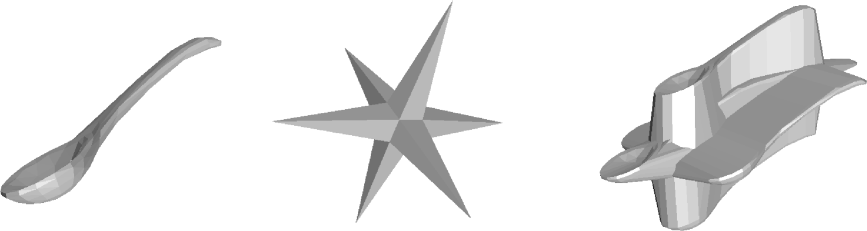
\includegraphics[width=0.9\textwidth]{Minkowski_sum_3/fig/spoon_star}
    \end{center}
  \end{ccTexOnly}
  \begin{ccHtmlOnly}
    <p><center>
    <img src="./fig/spoon_star.gif" border=0 alt="Minkowski sum
    example" width=700>
    </center>
  \end{ccHtmlOnly}
  \caption{The Minkowski sum of a spoon and a star.}
  \label{fig:spoonStar}
\end{figure}

The Minkowski sum of two point sets $P$ and $Q$ in $\mathbb{R}^d$, denoted by
$P \oplus Q$, is defined as the set $\{p+q:p \in P, q \in Q
\}$. Minkowski sums are used in a wide range of applications such as
robot motion planning~\cite{l-rmp-91} and computer-aided
design~\cite{cgal:ek-sicad-99}. Figure~\ref{fig:motionPlanning} shows
an example how Minkowski sums can be used to plan the motion of a
translational robot. We want to know which are legal positions of the
robot, and where can the robot go to from a specified starting
position. If we model both the robot and the obstacles as a polyhedron
and compute the Minkowski sum of the inverted robot (robot reflected
at the origin) and the obstacles, then this Minkowski sum represents
all illegal positions of the robot, i.e., all positions where it
intersects the obstacle. Of course, the complement of that polyhedron
describes all legal positions of the robot, i.e., all positions where
it does not intersect an obstacle.

\begin{figure}
  \begin{ccTexOnly}
    \begin{center}
      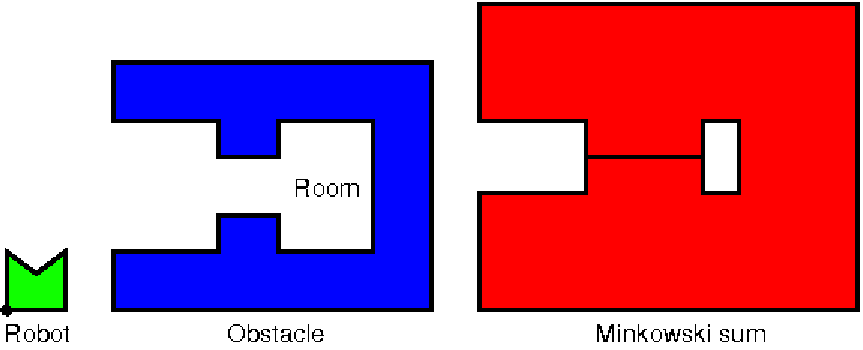
\includegraphics[width=0.8\textwidth]{Minkowski_sum_3/fig/motion_planning}
    \end{center}
  \end{ccTexOnly}
  \begin{ccHtmlOnly}
    <p><center>
    <img src="./fig/motion_planning.gif" border=0 alt="motion
    planning">
    </center>
  \end{ccHtmlOnly}
  \caption{Can the robot enter the room? The Minkowski sum of the inverted
           robot and the obstacle describes the illegal positions of the 
           robot with respect to the obstacle. 
           Since the boundary of the Minkowski sum describes legal
           positions, there
           is a path for the robot between the outer area and the room.}
  \label{fig:motionPlanning}
\end{figure}

The Minkowski sum can be illustrated as follows. Pick an arbitrary
reference point $r$ of $P$ (black dot in the lower left corner of the
robot in Figure~\ref{fig:motionPlanning}). Then place the inverted set
$-P$ on $Q$, such that $-r$ is on the boundary of $Q$. Finally, move
$-P$ along the complete boundary of $Q$. The union of $Q$ and the
points swept by $-P$ is the Minkowski sum of $P$ and $Q$.

Implementing the Minkowski sum, the reference point does not need to
be chosen. It is implicitly given as the origin of the coordinate
system. Choosing a different reference point is equivalent to
translating the coordinate system. Such a translation does not change
the shape of the Minkowski sum; it only translates the Minkowski sum
by the same vector.

This package provides a function \ccc{minkowski_sum_3} that computes
the Minkowski sum of two Nef polyhedra. We do not support arbitrary
Nef polyhedra, yet. The restrictions are discussed in detail in
Section~\ref{sectionMinkowskiSum_3Restrictions}.

% +------------------------------------------------------------------------+
\section{Decomposition Method}

The decomposition method for computing the Minkowski sum of non-convex
polyhedra makes use of the fact that Minkowski sums of convex
polyhedra are rather easy to compute. It decomposes both polyhedra
into convex pieces, computes all pairwise Minkowski sums of the convex
pieces, and merges the pairwise sums~\cite{bkos-cgaa-97}.

\begin{figure}[t]
  \begin{ccTexOnly}
    \begin{center}
      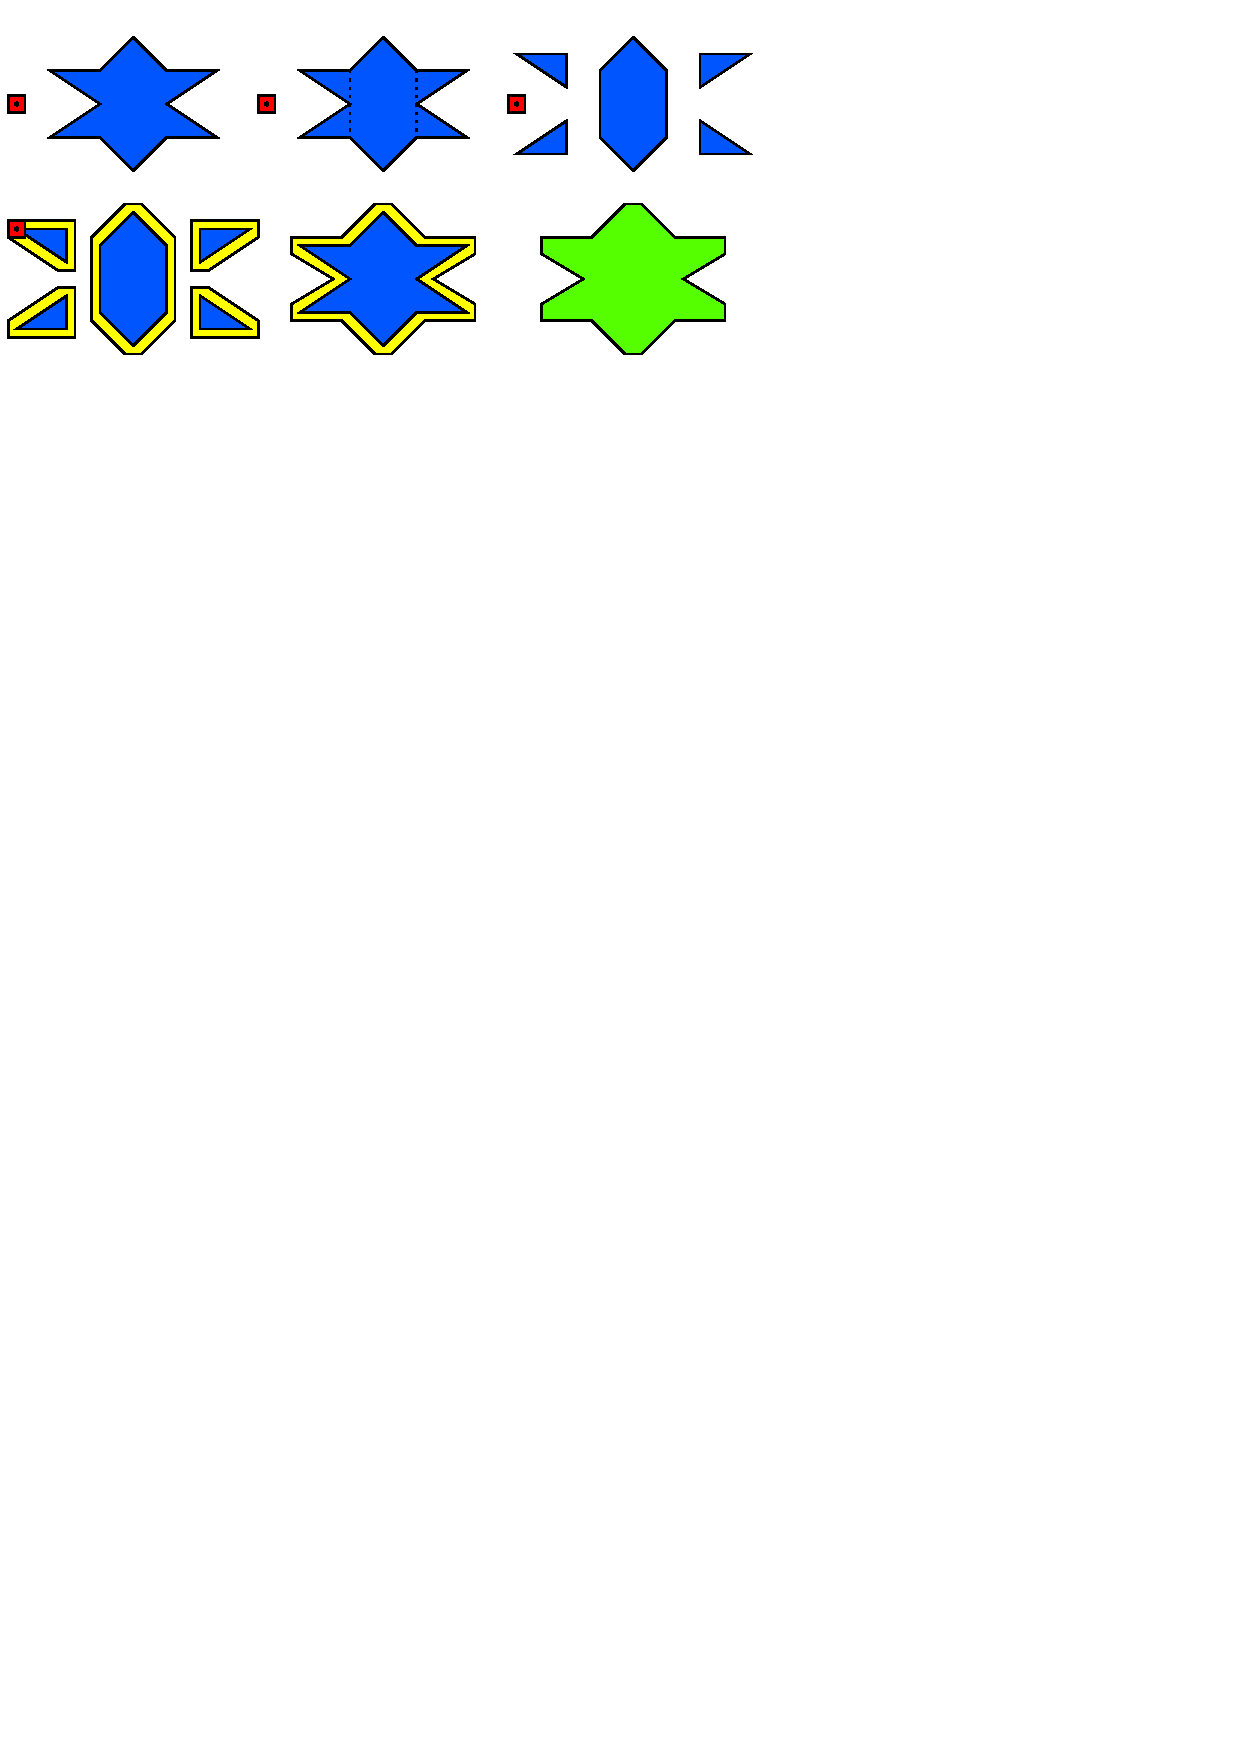
\includegraphics[width=0.8\textwidth]{Minkowski_sum_3/fig/decomposition_method}
    \end{center}
  \end{ccTexOnly}
  \begin{ccHtmlOnly}
    <p><center>
    <img src="./fig/decomposition_method.gif" border=0
    alt="decomposition method" width=700>
    </center>
  \end{ccHtmlOnly}
  \caption{The decomposition method decomposes both input polyhedra
           into convex parts, computes all pairwise Minkowski sums
           of the convex parts, and merges the pairwise sums.}
\end{figure}

Minkowski sum are inherently complex to compute. Using the
decomposition method, each polyhedron might be divided into a
quadratic number of pieces, which is worst-case optimal. Then up to
$n^2m^2$ pairwise sums have to be computed and merged, where $n$ and
$m$ are the complexities of the two input polyhedra (the complexity of
a \ccc{Nef_polyhedron_3} is the sum of its \ccc{Vertices},
\ccc{Halfedges} and \ccc{SHalfedges}). In total the operation runs in
$O(n^3m^3)$ time.

Since the computation of the Minkowski sum takes quite some time, we
give the running times of some Minkowski sum computations. They were
computed with \cgal\ 3.3 on a machine with a 2.4 GHz AMD Opteron
processor and 4 GB RAM. The code was compiled with
g++ 3.2 and compiler options -O2. The
\ccc{Nef\_polyhedron\_3} class was instantiated with the geometric
kernel \ccc{Homogeneous<leda_integer>}. The Minkowski sum of the spoon
and the star is illustrated in Figure~\ref{fig:spoonStar}.

\begin{table}[h]
\begin{center}
\begin{tabular}{|ccc|ccc|c|}
\hline
\multicolumn{3}{|c|}{model 1} & \multicolumn{3}{|c|}{model 2} & running \\
name & facets & conv. pcs. & name & facets & conv. pcs. & time \\ 
\hline
mushroom & 448 & 255 & cube & 6 & 1 & 204s \\
mushroom & 448 & 255 & ball1 & 128 & 1 & 553s \\
spoon & 336 & 186 & star & 24 & 5 & 882s \\
cup & 1000 & 774 & ball2 & 1000 & 1 & 9851s \\
\hline
\end{tabular}
\caption{Performance of the function \ccc{minkowski_sum_3}.}
\end{center}
\end{table}

% +------------------------------------------------------------------------+
\section{Features and Restrictions}
\label{sectionMinkowskiSum_3Restrictions}

This package was written to allow the computation of Minkowski sums of
full-dimensional polyhedra even in so-called tight-passage scenarios.
Tight passage scenarios occur in robot motion planning, when a robot
is just as wide as a passage it needs to traverse. In these scenarios
at least one polyhedron---the obstacles or the robot---must be modeled
as an open set. Then the Minkowski sum will also be an open set and
tight passages will occur as lower-dimensional exclusions, i.e., as
facets, lines, or vertices that are, in contrast to the volume around
them, not part of the resulting point
set. Figure~\ref{fig:motionPlanning} shows such a tight passage
scenario.

Our implementation uses \ccc{Nef_polyhedron_3} to model the input
polyhedra and the result polyhedron. An instance of
\ccc{Nef_polyhedron_3} represents a subdivision of the
three-dimensional space into vertices, edges, facets, and
volumes. Some of these items form the polyhedron (selected), while
others represent the outer volume or holes within the polyhedron
(unselected). As an example, the unit cube is the point set
$[0,1]^3$. The smallest subdivision that represents the unit cube has
8 vertices, 12 edges, 6 facets, and 2 volumes. The volumes enclosed by
the vertices, edges, and facets is the interior of the cube and
therefore selected. The volume outside the cube does not belong to it
and is therefore unselected. The vertices, edges, and facets---also
denoted as boundary items---are needed to separate the two volumes,
but are also useful for representing topological properties. In case
of the (closed) unit cube the boundary items are part of the
polyhedron and therefore selected, but in case of the open unit cube
$[0,1)^3$ they are unselected. Each item has its own selection mark,
which allows the correct representation of Nef polyhedra, which are
closed under Boolean and topological operations. Details can be found
in the chapter on 3D Boolean operations on Nef polyhedra~\ref{chapterNef3}.

The use of \ccc{Nef_polyhedron_3} allows many scenarios beyond the
Minkowski sum of two solids. First, they can model the input and the
result of a tight passage scenario, i.e., they can model open and
closed solids as is needed for the input models, and they can model
tight passages, which are lower-dimensional exclusions represented as
unselected facets, edges, and vertices. We strive for extending the
package to work for arbitrary 3D Nef polyhedra. In addition to the
Minkowski sums of two solids, we added several features. At the moment
we allow an input polyhedron to consist of:
\begin{enumerate}
\item singular vertices
\item singular edges
\item singular convex facets without holes
\item surfaces with convex facets that have no holes.
\item three-dimensional features, whose coplanar facets have
common selection marks (this includes open and closed solids)
\end{enumerate}

Taking a different viewpoint, the implementation is restricted as
follows:
\begin{enumerate}
\item The input polyhedra must be bounded (selected outer volume is ignored).
\item All sets of coplanar facets of a full-dimensional
feature must have the same selection mark (in case of different
selection marks, unselected is assumed).
\item All facets of lower-dimensional features need to be convex and 
must not have holes (non-convex facets and holes are ignored).
\end{enumerate}

The second restriction might seem a bit odd. It stems from the fact
that the Minkowski sum on convex polyhedra can only handle polyhedra,
whose sides consist of a single facet. The decomposition process
usually yields complex adjacency relations between a convex part, its
adjacent convex parts, and the outer volume. The side of a convex
piece is then decomposed into several facets, each of which represents
one of these adjacency relations. For the convex Minkowski sum, we
ignore the decompositions of the sides, but need to find a common
selection mark. If there are two facets that are adjacent to the outer
volume, but have different selections marks, we cannot set a common
selection mark without spoiling the correctness of the Minkowski sum.

% +------------------------------------------------------------------------+
\section{Usage}

The function \ccc{minkowski_sum_3} should be used with the
\ccc{Exact_predicates_exact_constructions_kernel}, which often is
the most efficient choice and allows floating-point input. Consult
Section~\label{sectionNef_3IO} for more details.

The following example code illustrates the usage of the function
\ccc{minkowski_sum_3}. Note that either input polyhedra will be
modified by the function if it is non-convex. So, if they are needed
further on, they need to be copied, first. The copying is not done by
the function itself to keep the memory usage as small as possible.

\ccIncludeExampleCode{Minkowski_sum_3/cube_offset.cpp}

% +------------------------------------------------------------------------+
\section{Glide}

\begin{figure}
  \begin{center}
    \begin{ccTexOnly}
      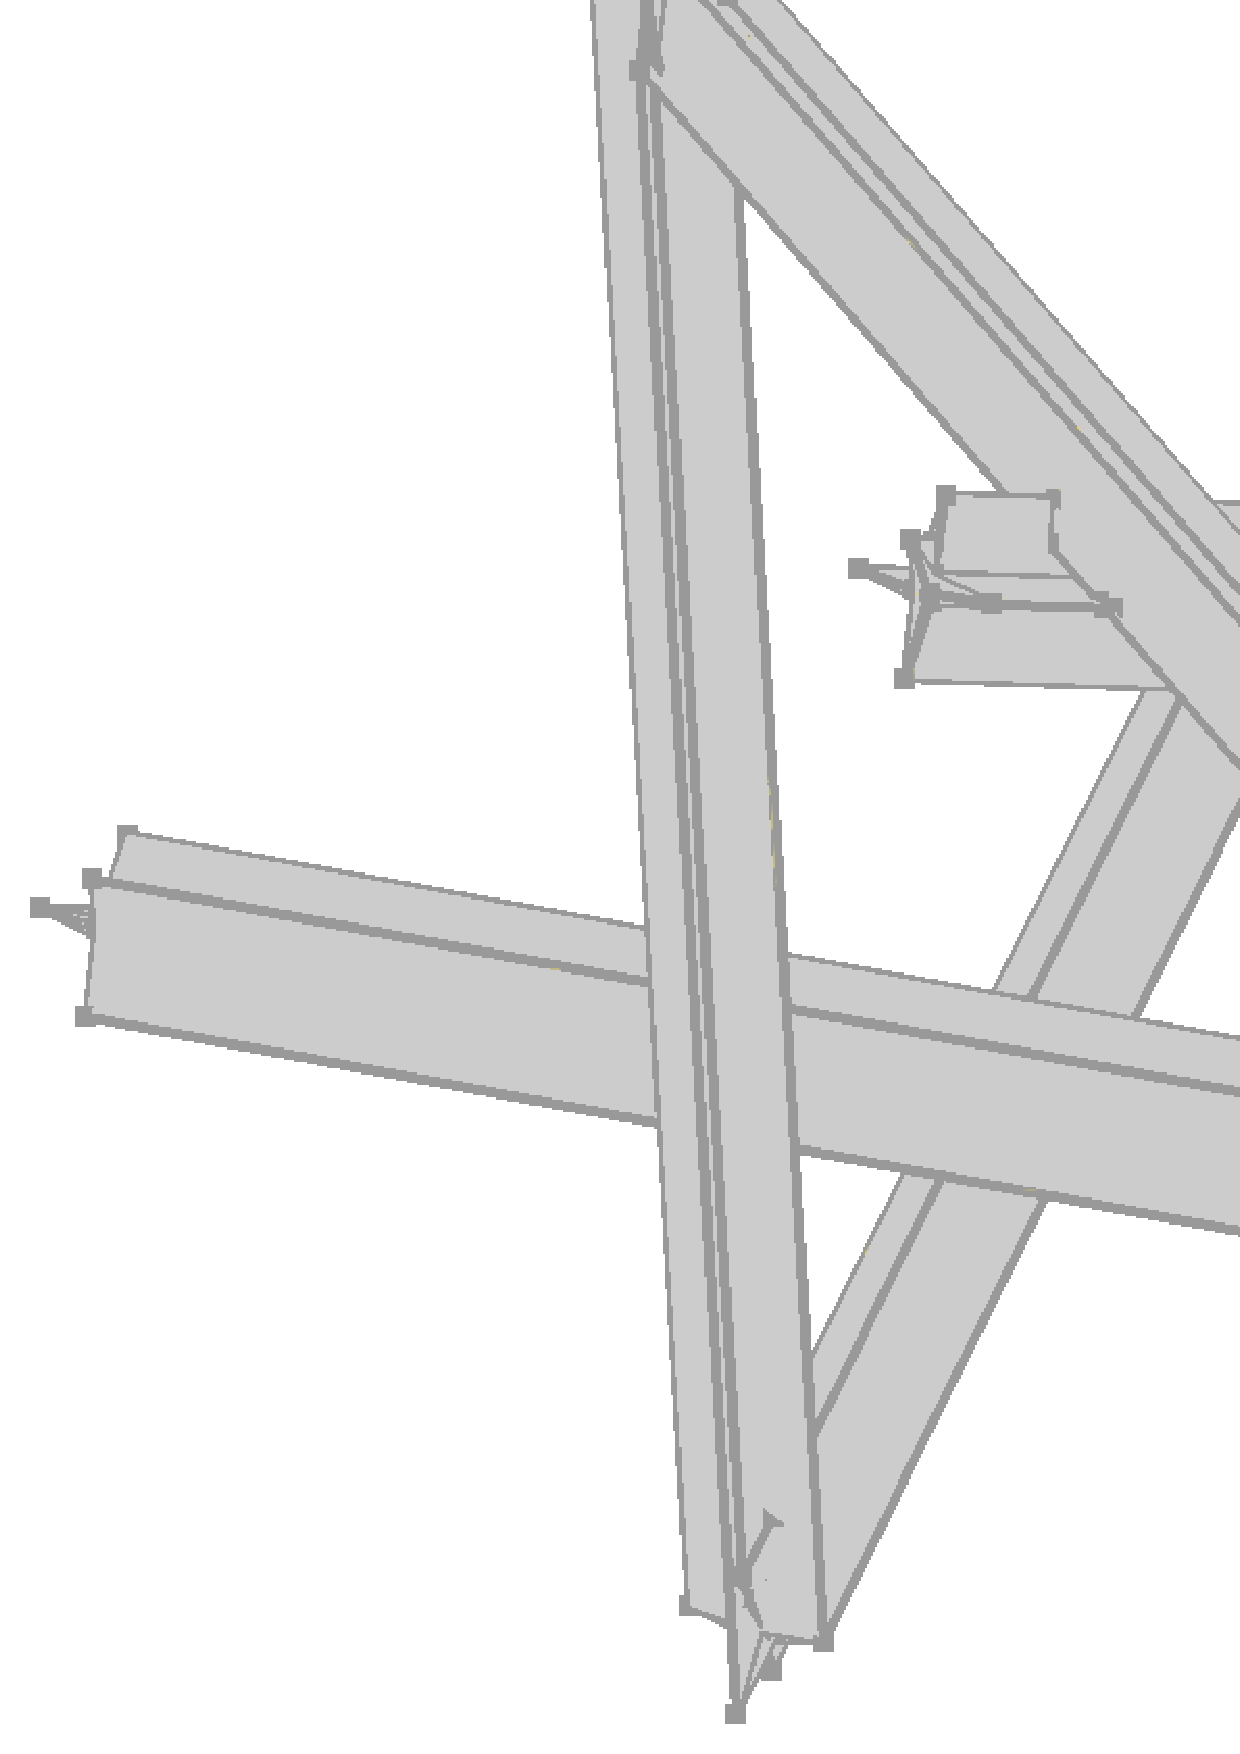
\includegraphics[width=0.5\textwidth]{Minkowski_sum_3/fig/glide}

  \end{ccTexOnly}
  \begin{ccHtmlOnly}
    <img src="./fig/glide.gif" border=0 alt="glide operation" width=400>
  \end{ccHtmlOnly}
    \end{center}
  \caption{The region swept by a star that moves along a polygonal path.}
\end{figure}

With the function \ccc{minkowski_sum_3} it is also possible to realize
other interesting geometric operations like the glide operation, which
computes the point set swept by a polyhedron that moves along a
polygonal path. The following example shows how to construct a
polygonal path and then compute the glide operation by calling the
function \ccc{minkowski_sum_3}.

\ccIncludeExampleCode{Minkowski_sum_3/glide.cpp}
